\section{Multi-Stage Ensemble}
Stratified 5-fold cross validation (CV).
We used xgboost \cite{xgboost}, neural nets and linear regression for stage-II ensembling.

\begin{figure}[!ht]
  \caption{5-fold CV stacked generalization ensemble}
  \centering
    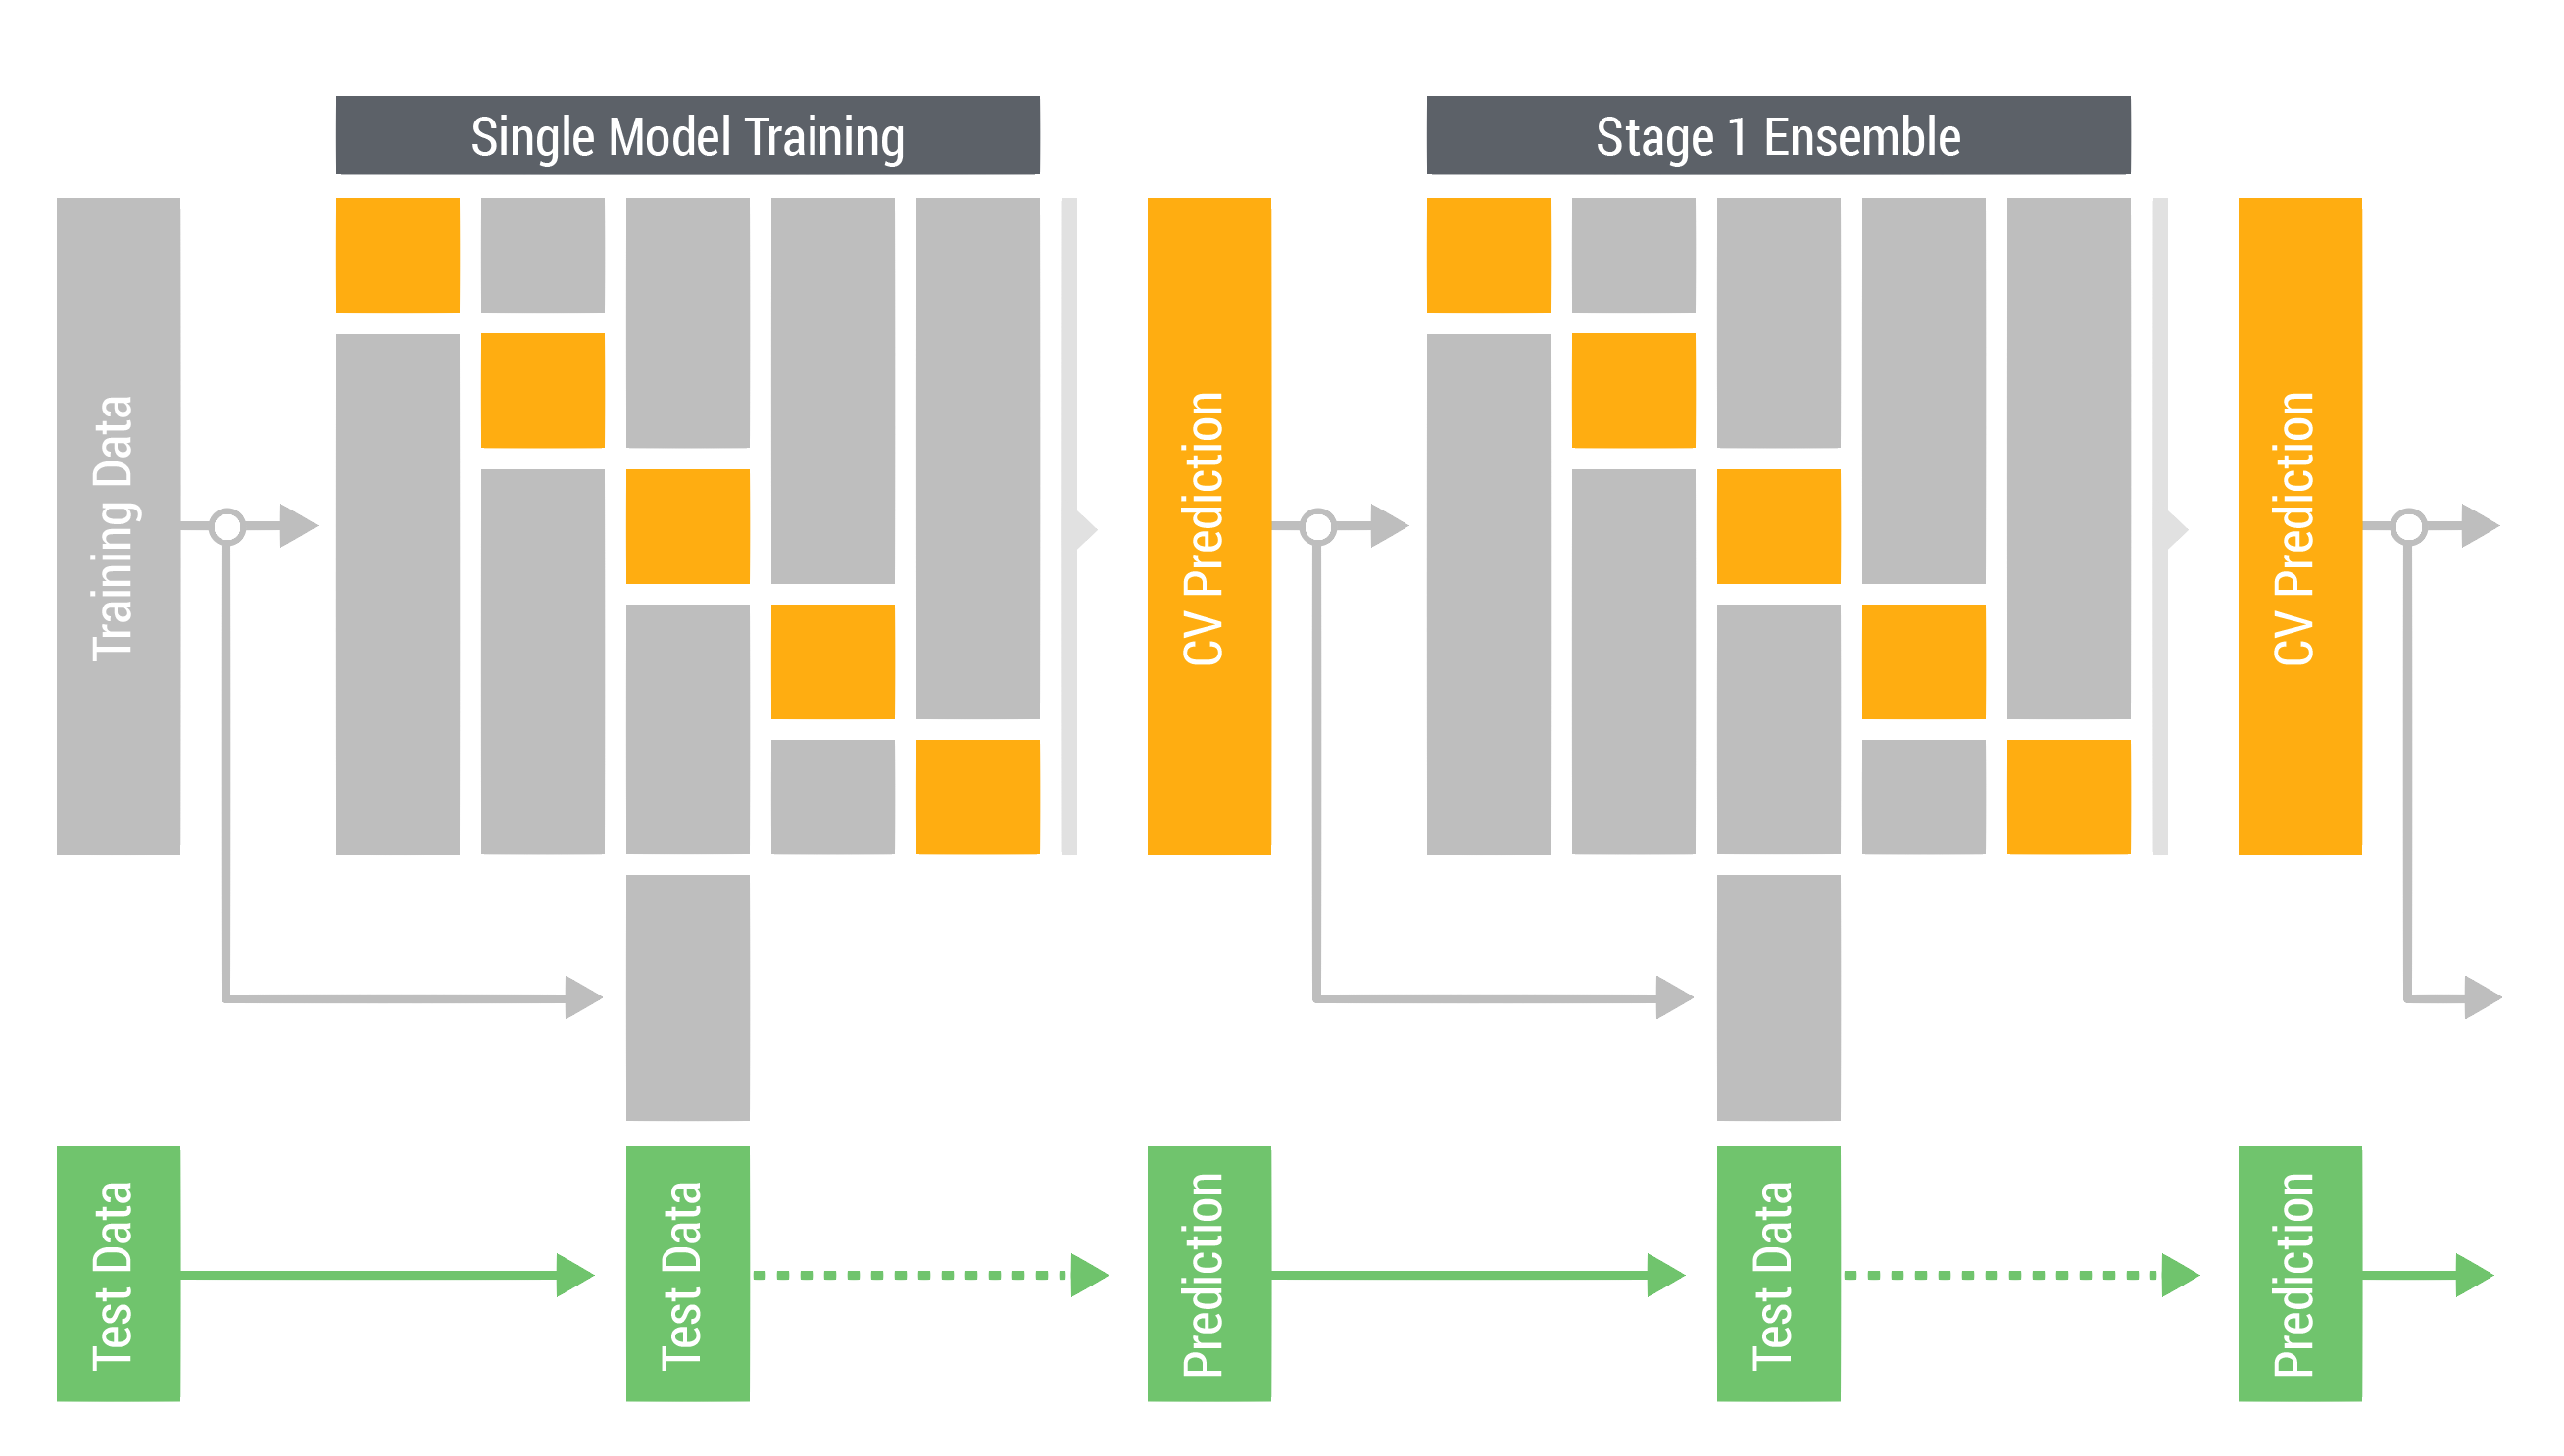
\includegraphics[width=0.5 \textwidth]{cv_ensemble}
\end{figure}

\begin{figure*}[!ht]
  \caption{End-to-end pipeline for the final solution}
  \centering
    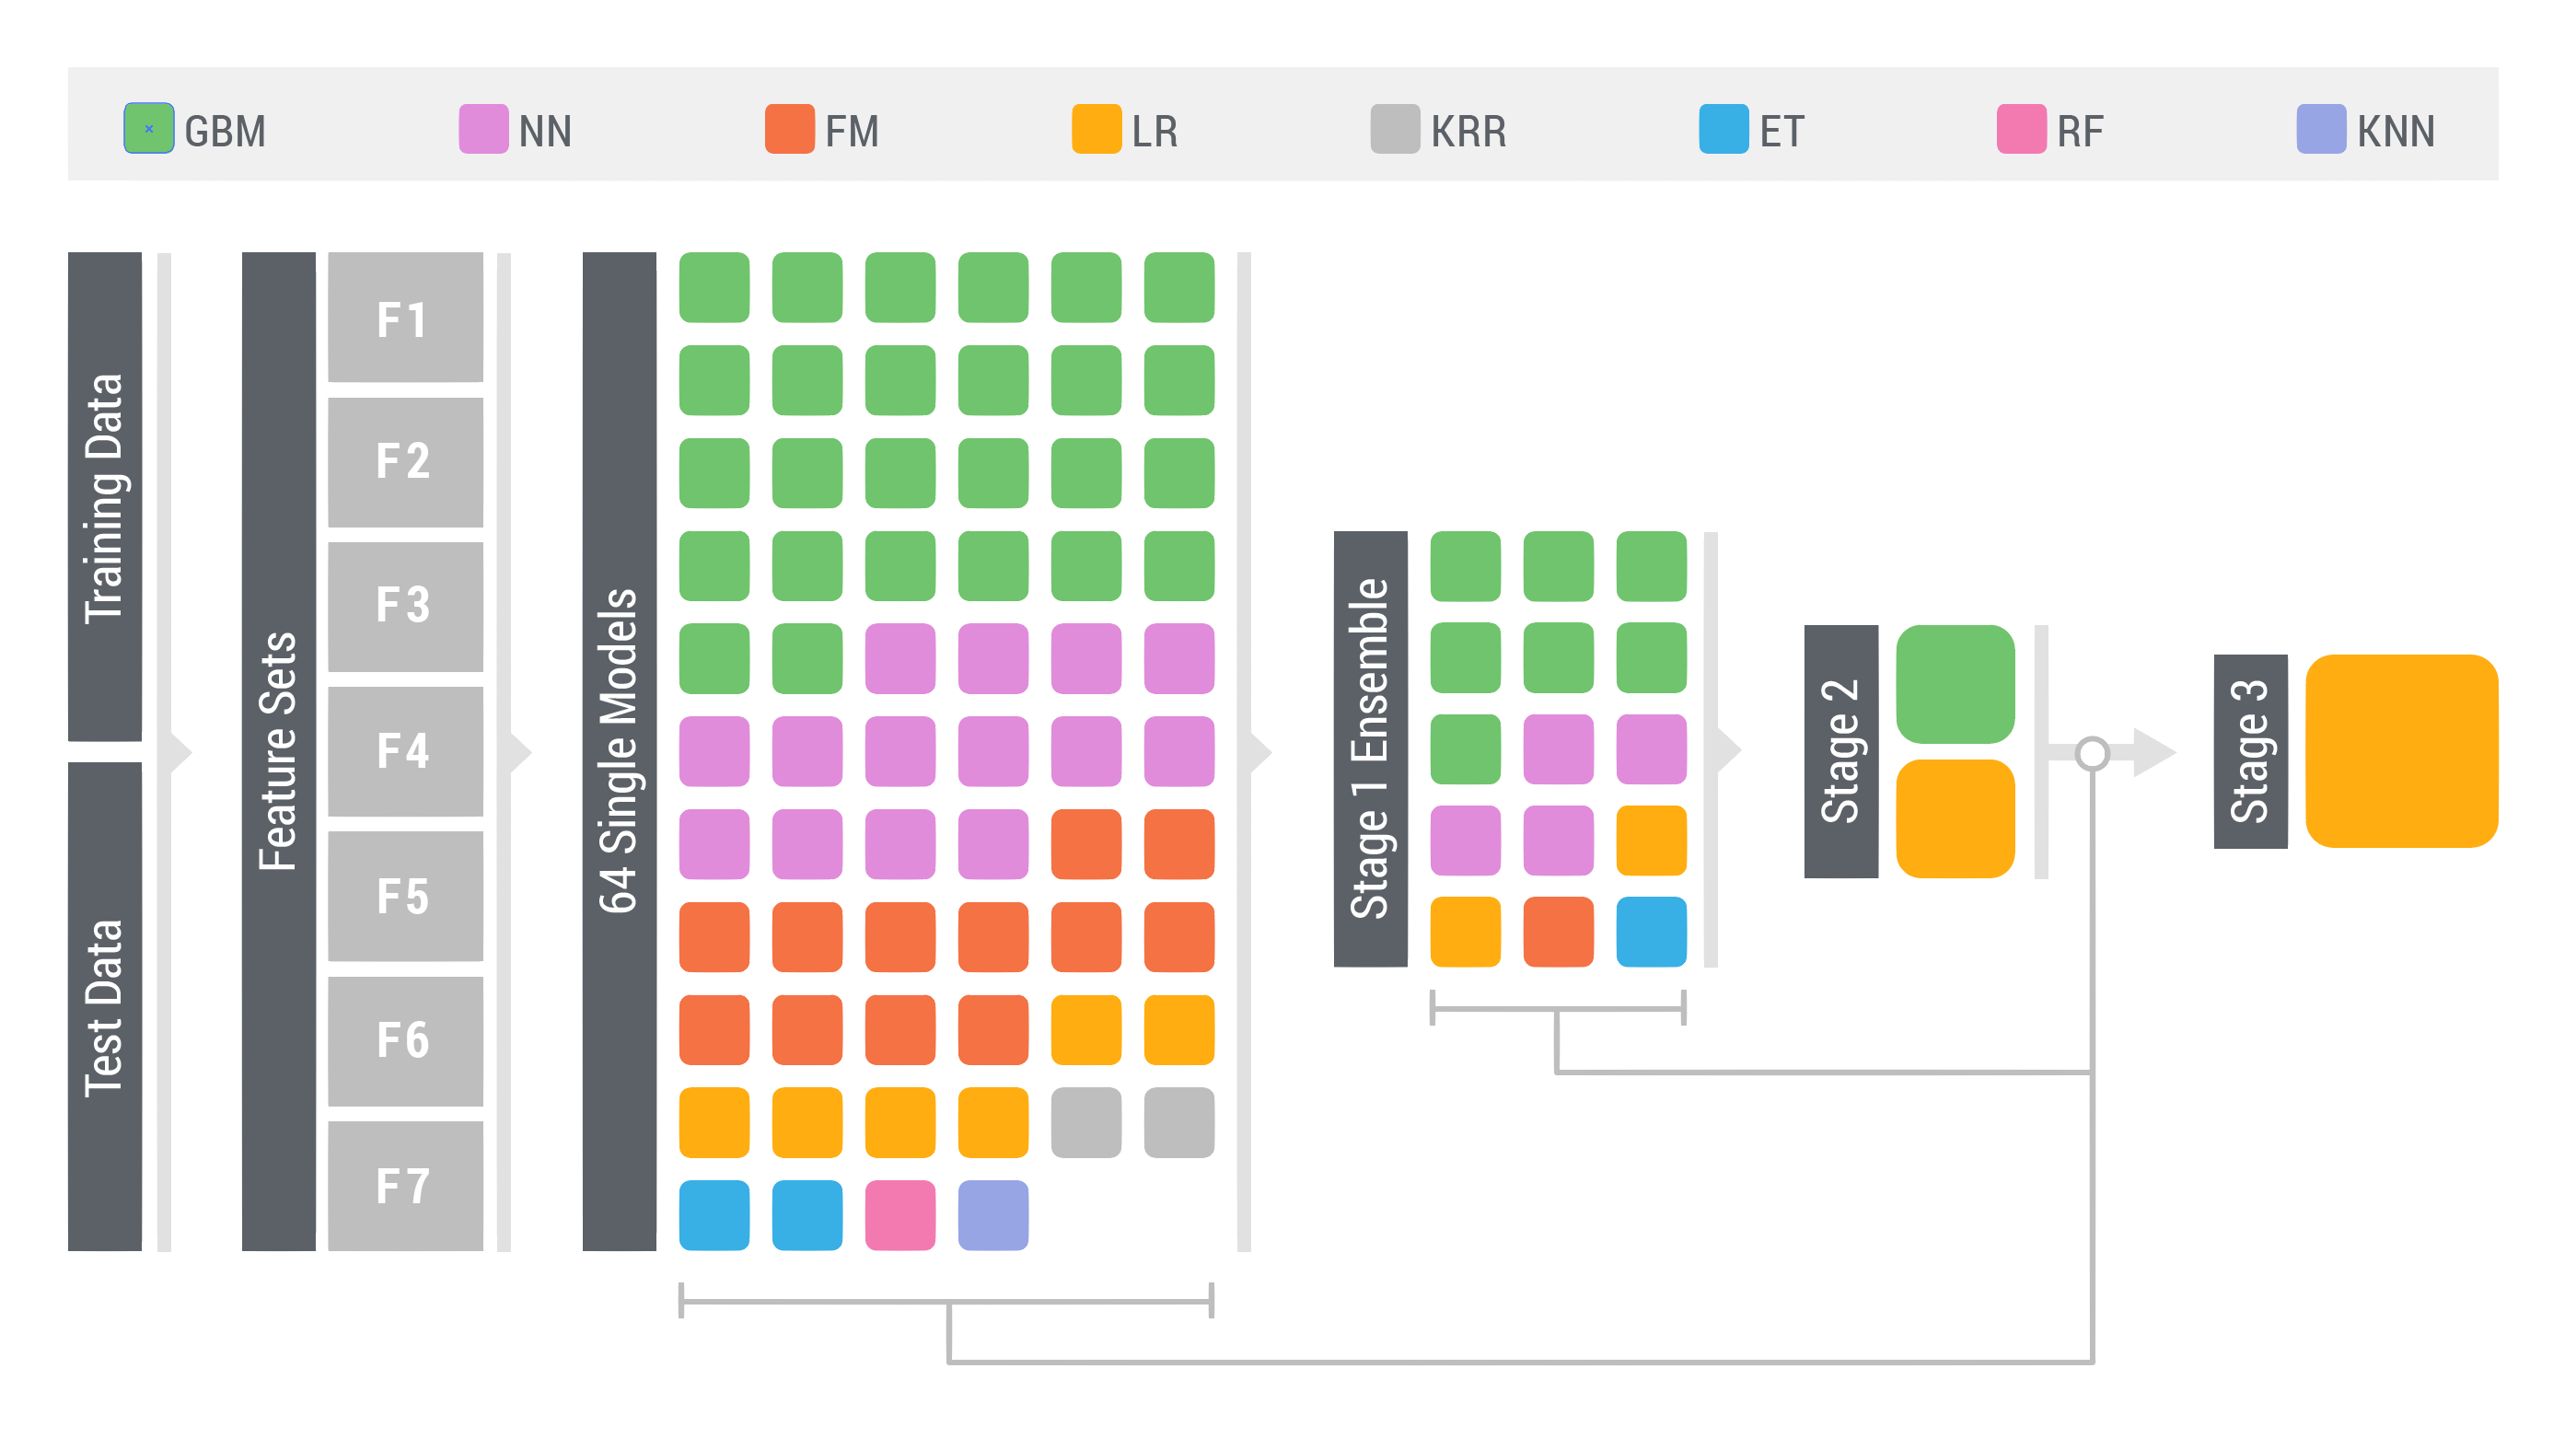
\includegraphics[width=1 \textwidth]{ensemble}
\end{figure*}

\begin{figure*}[!ht]
  \caption{5-fold CV vs. public leaderboard AUC scores}
  \centering
    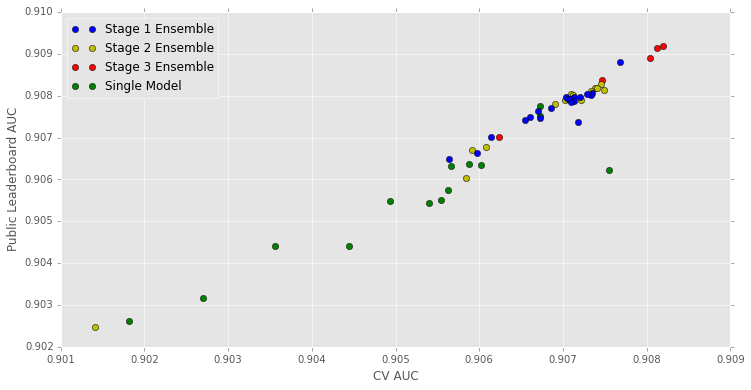
\includegraphics[width=1 \textwidth]{cv_lb}
\end{figure*}

\subsection{Stage-I Ensemble}
We trained 15 stage-I ensemble classifiers with different subsets of CV predictions of 64 individual classifiers.

\subsection{Stage-II Ensemble}
We trained 2 stage-II ensemble classifiers with different subsets of CV predictions of 15 stage-I ensemble classifiers.

\subsection{Stage-III Ensemble}
We trained a stage-III ensemble classifier with CV predictions of 5 classifiers: 1 stage-II ensemble, 3 stage-I ensemble, and 1 individual classifiers.
\\

\begin{center}
\begin{tabular}{lllll}
\label{tb:finalEnsemble}
ID 	& Model 				& Type 	& 5-CV 		& Weight\\ \hline
S1 	& xgb\_rf.ko\_new\_feat 	& Single 	& 0.906721 	& 1.1703 \\
E4 	& at.esb50v2+ko 		& Stage I 	& 0.907878 	& 1.9626\\
E8 	& esb58v5+magic.dae+nn & Stage I & 0.907567	& 0.7871\\
E18	& et\_esb58v5\_rank		& Stage I	& 0.906207 	& 0.4580\\
E2	& lr\_forward\_0.01\_esb.esb15v3 & Stage II & 0.907968 & 1.6146\\
\end{tabular}
\end{center}

A linear combination of the 5 models from table \ref{tb:finalEnsemble} results in train AUC=0.908072 and accuracy=0.887334.
Which leads to 0.90910 public leaderboard score.
By adding 39 courseID correction factors train AUC=0.908194 and public score improved to 0.90918.

%final ensemble:
%Read 1|5  trn.final.90788  acc:0.887135  AUC:0.907878
%Read 2|5  esb58v5+magic.dae+nn.validCV.0.907567  acc:0.887143  AUC:0.907567
%Read 3|5  et_esb58v5_rank.val.0.906207  acc:0.886919  AUC:0.906207
%Read 4|5  lr_forward_0.01_esb.esb15v3.val.yht  acc:0.887276  AUC:0.907968
%Read 5|5  xgb_rf.ko_new_feat.txt.valCV.0.906721  acc:0.886753  AUC:0.906721
%linear weights:
%w0=1.96267 w1=0.787138 w2=0.458095 w3=1.61461 w4=1.1703
%final train errors:
%acc:0.887334 AUC:0.908072
%by adding course correction factors AUC on train improved to 0.908194

%Finally we ended up with linear ensembling with 39 courseID correction factors.
%These 39 factors improved the score from 0.90910 to 0.90918.

\begin{table*}[t]
\begin{center}
\begin{tabular}{lllll}
\label{tb:ensembleModels}
ID	& Stage	& Model 				& 5-CV		& Public Leaderboard \\ \hline
E1	& III		& subBlend\_0712v2		& 0.908194 	& 0.909181 \\
E2	& II		& lr\_forward\_0.01\_esb.esb15v3 & 0.907968	& - \\
E3	& II		& xgl\_10\_0.01\_10\_10\_esb.esb11v6 & 0.907379 & 0.908187 \\
E4 	& I		& at.esb50v2+ko			& 0.907878	& - \\
E5	& I		& xg\_sk\_1800\_5\_0.004\_esb51\_rank & 0.907734 \\
E6 	& I		& lr\_forward\_0.01\_esb51\_rank\_norm & 0.907716	& - \\
E7	& I		& song\_train\_xgb\_esb58v5\_ko & 0.907668	& 0.908796 \\
E8	& I		& esb58v5+magic.dae+nn		& 0.907567	& - \\
E9	& I		& esb58v3.trn.final			& 0.907353	& 0.908060 \\
E10	& I		& trn.esb56.blend.at			& 0.907283	& 0.908043 \\
E11 	& I		& ConfigAMLCUDAPreModel	& 0.907076	& - \\
E12	& I		& xg\_sk\_1800\_5\_0.004\_esb56\_rank\_4 & 0.907036	& 0.907977 \\
E13 	& I		& esb55.dae+nn			& 0.906956	& - \\
E14	& I		& lr\_0.01\_esb51\_rank\_norm	& 0.906746	& - \\
E15 	& I		& nn						& 0.906714	& - \\
E16	& I		& xgb\_rf\_esb55.xix			& 0.906689	& - \\
E17	& I		& libfm					& 0.906537	& - \\
E18 	& I		& et\_esb58v5\_rank			& 0.906200	& - \\
\end{tabular}
\end{center}
\end{table*}
